\documentclass{hsflensburg}
\title{Wissenschaftliche Ausarbeitung}
\subtitle{PHOABE: Policy-Hidden Outsourced Attribute Based Encryption}

% Authors
\author{
	\name{Florian Hansen}\\
  \institution{Hochschule Flensburg}
}

% Packages
\usepackage[utf8]{inputenc}
\usepackage[ngerman]{babel}
\usepackage{amsthm}
\usepackage{amsmath}
\usepackage{amssymb}
\usepackage{kbordermatrix}

\newtheorem{definition}{Definition}
\newtheorem*{example}{Beispiel}
\renewcommand{\kbldelim}{(}
\renewcommand{\kbrdelim}{)}

\newcommand{\algitem}[4]{\textbf{$\text{#1}_{#2}\left({#3}\right) \to {#4}$.}\;\;\;\;}


\begin{document}
	\maketitle
	\begin{abstract}
	\end{abstract}

	\section{Einleitung}
	Diese wissenschaftliche Ausarbeitung wird im Rahmen der Hochschulveranstaltung
	\textit{Hot-Topics in der IT-Security} angefertigt und handelt über den
	sicheren Datenaustausch zwischen Internet-of-Things-Geräten.  Besonders wird
	hierbei auf die Attribute Based Encryption (ABE) eingegangen, welche ein
	relativ junges Forschungsgebiet der Kryptographie darstellt. Es existieren
	zwar einige ABE-Schemata, diese sind jedoch für leistungsschwache Geräte eher
	ungeeignet.

	Diese Ausarbeitung beschäftigt sich hauptsächlich mit der Arbeit von
	\cite{phoabe}, welche ein neues attribut-basiertes Verschlüsselungsschema
	vorstellt: \textit{PHOABE}. Dieses Schema widmet sich bekannten Problemen der
	Attribut-basierten Verschlüsselung, wie zum Beispiel das Verstecken der
	Zugriffsregelungen (\textit{Access-Policies}), die sensitive Daten enthalten
	können. Zusätzlich fordert das Schema eine Auslagerung des
	Entschlüsselungsvorganges, welches aufgrund von bilinearen Abbildungen relativ
	rechenintensiv ist. Hierbei sollen sogenannte \textit{Semi-trusted Cloud
	Server} den aufwändigen Teil der Berechnung über\-nehmen, damit auch
	leistungsschwache Geräte solche attribut-basierte Ver\-schlüs\-sel\-ung\-en
	durchführen können.

	\section{Problembeschreibung}
	Das \textit{Internet der Dinge}, \textit{Internet of Things} (IoT), hat die
	Aufgabe, verschiedenste Hardwarekomponenten miteinander zu verbinden und damit
	einen Datenaustausch zu ermöglichen. Ein gutes Beispiel hierfür sind
	Smartphones und Sensoren, die ständig miteinander kommunizieren müssen bzw.
	sollen. Grundsätzlich können IoT-Anwendungen aufgrund ihrer
	Kommunikationsfähigkeit in zwei Bereiche eingeteilt werden. In
	Einzelanwendungen be\-nö\-ti\-gen man lediglich eine Autorität während es auch
	Anwendungsfälle gibt, die über unterschiedliche Bereiche bzw. Domänen
	kommunizieren müssen. Diese besitzen damit mehrere Autoritäten \cite{phoabe}.

	Beide Klassen von IoT haben eins gemeinsam. Sie müssen einen sicheren Austausch
	von Daten und die Sicherung der Privatsphäre gewährleisten. Hierfür werden
	Daten verschlüsselt und mithilfe von Zugriffskontrollmechanismen nur
	bestimmten Parteien zur Verfügung gestellt. Genau deshalb ist die
	attribut-basierte Verschlüsselung ein attraktiver Kandidat, da sie
	Zugriffskontrolle (\textit{Access-Control}) und Verschlüsselung miteinander
	verknüpft. Ein Problem dabei exisitiert dennoch. Dieses Verfahren verwendet
	bilineare Abbildungen, was vor allem in der Entschlüsselung viel Rechenaufwand
	bedeutet. Für leistungsstarke Desktop-Rechner mag dies weniger eine Rolle
	spielen, ist jedoch bezogen auf IoT ein großes Problem, denn dort
	kommunizieren in der Regel Geräte mit sehr eingeschränkten Ressourcen
	miteinander. Zudem erhöht sich der Rechenaufwand proportional zur Anzahl
	der Attribute. Das Problem liegt also darin, Daten sicher und effizient
	zwischen ressourcenarmen Geräten auszutauschen, ohne die Privatsphäre der
	Benutzer zu verletzen.

	\section{Motivation}
	Die attribut-basierte Verschlüsselung ist, wie in der Problembeschreibung
	bereits erwähnt, ineffizienter, je mehr Attribute verwendet werden. Besonders
	die Entschlüsselung wird durch die bilinearen Operationen extrem
	rechenaufwändig, was zur Folge hat, dass dieses Schema auf ressourcenärmeren
	Geräten und damit auf IoT nur bedingt anwendbar ist. Eine wichtige Frage, die
	sich also stellt ist, wie man ABE für eben solche Anwendungsfälle anwendbar
	gestalten kann.

	In weiterführenden Arbeiten, so auch der von \cite{green}, wird ein neues
	Konzept in Verbindung mit attribut-basierter Verschlüsselung vorgestellt, um
	diese effizienter zu gestalten. Für die kostspielige Entschlüsselung ist nun
	nicht mehr alleine der jeweilige Benutzer zuständig, sondern eine weitere
	Instanz. Ein halb vertrauenswürdiger Cloud-Server (\textit{semi-trusted cloud
	server}, STCS), welcher den rechenaufwändigen Teil der Entschlüsselung
	übernehmen soll. Damit der Server keinerlei Informationen über den
	entschlüsselten Ciphertext erhält, soll dieser diesen lediglich zum Teil
	entschlüsseln.  Anschließend wird das Ergebnis vom Benutzer selbst
	entschlüsselt. So soll garantiert werden, dass die rechenaufwändige Arbeit vom
	STCS und nicht vom Benutzer übernommen wird und trotzdem keinerlei
	Informationen über die eigentliche Nachricht an dem Server preisgegeben wird.

	Eine weitere Überlegung von \cite{phoabe} ist folgende. Was ist, wenn der STCS
	das teilweise entschlüsselte Chiffrat fälscht? Es muss also zusätzlich die
	Möglichkeit bestehen, dass das Ergebnis der Entschlüsselung des STCS'
	überprüft werden kann. Einige vergangene Arbeiten haben sich dem Problem
	gewidmet, jedoch keine effiziente Lösung geboten oder sind inpraktikabel für
	IoT, da sie sich auf einer einzigen Autorität stützen. Da IoT jedoch
	hauptsächlich über mehrere Domänen kommuniziert, ist dies keine praktikable
	Lösung. Die Motivation hinter \cite{phoabe} ist also, ein ausgelagertes,
	verifizierbares multi-authority ABE-Schema zu entwerfen.
	
	\section{Grundlagen}
	\subsection{Zugriffsregeln}
	Grundsätzlich werden Regeln für den Datenzugriff durch zwei Formate
	repräsentiert. Zum Einen durch boolsche Funktionen und zum Anderen durch
	sogenannte Linear Secret Sharing Schemes (LSSS). In diesem Abschnitt sollen
	beide Repräsentationsmöglichkeiten eingeführt werden.

	\begin{definition}[Zugriffsstrukturen \cite{abe}]\label{def:access-structures}
		Sei $\left\{ P_1, P_2, ..., P_n \right\}$ die Menge der beteiligten
		Parteien. Eine Sammlung $\mathbb{A} \subseteq 2^{\left\{ P_1, P_2, ..., P_n
		\right\}}$ ist monoton, wenn $\forall B, C .\;\; B \in \mathbb{A}
		\;\;\land\;\; B \subseteq C \implies C \in \mathbb{A}$. Eine
		Zugriffsstruktur ist damit eine Sammlung $\mathbb{A}$ von nicht-leeren
		Untermengen von dem Universum $\left\{ P_1, P_2, ... P_n \right\}$. Alle
		Mengen $A \in \mathbb{A}$ werden als authorisierte Mengen während
		die nicht in $\mathbb{A}$ vertetenden Mengen als unauthorisierte
		bezeichnet werden.
	\end{definition}

	Definition ~\ref{def:access-structures} kann dabei so interpretiert werden,
	als dass alle Obermengen jedes Elements $B \in \mathbb{A}$ verteten sein
	müssen. Im Folgenden soll ein Beispiel dies verdeutlichen.

	\begin{example}
		Sei $\mathbb{U} = \left\{ 1, 2, 3, 4 \right\}$ ein Universum und $\mathbb{A}
		\subseteq 2^\mathbb{U}$ eine Zugriffsstruktur.

		Die Zugriffsstruktur $\mathbb{A} = \left\{ \left\{1,2\right\},
		\left\{3,4\right\} \right\}$ ist nicht monoton, da das Element
		$\left\{1,2,3\right\}$ nicht vorhanden ist.

		Die Zugriffsstruktur $\mathbb{A} = \left\{ \left\{3,4\right\},
		\left\{1,3,4\right\}, \left\{1,2,3,4\right\} \right\}$ ist monoton, da alle
		Obermengen der Elemente von $\mathbb{A}$ vorhanden sind.
	\end{example}

	\begin{definition}[Linear Secret-Sharing Schemes \cite{abe}]
		Ein Linear Secret-Sharing Scheme (LSSS) über eine Menge von Parteien $P$ ist
		linear, wenn

		\begin{enumerate}
			\item Die Anteile (shares) für jede Partei einen Vektor $\vec{v} \in
				\mathbb{Z}_p^{n+1}$ formen.
			\item Eine Matrix $M$ existiert, die $l$ Zeilen und $n+1$ Spalten enthält.
				Jede $i$-te Zeile aus $M$ mit $i \in \left\{1, ..., l\right\}$ ist dann
				mit einer Partei $x_i \in P$ beschriftet. Wenn wir den Spaltenvektor $v =
				\left(s, r_1, r_2, ..., r_n\right)$ betrachten, wobei $s \in \mathbb{Z}_p$ das zu
				teilende Geheimnis ist und $r_1, ..., r_n \in \mathbb{Z}_p$ zufällig
				gewählt werden, dann ist $Mv$ ein Vektor bestehend aus $l$ Anteilen des
				Geheimisses $s$.
		\end{enumerate}
	\end{definition}

	\begin{example}
		Gegeben sei eine LSSS-Matrix $M \in \mathbb{Z}_2^{l \times n}$ und die Abbilding $\rho : \mathbb{N^+}
		\times \mathbb{Z}_p^{l \times n} \to \mathbb{Z}_p^n$, welche die
		$i$-te Zeile der Matrix $M$ zurückgibt. Zudem werden den Zeilen Parteien
		$P_i$ zugewiesen, sodass $\rho(i, M)$ den Anteil der jeweiligen Partei liefert.
		$$M = \kbordermatrix{
				  &   &   &   \\
			P_2 &1 & 1 & 0 & 1 \\
			P_2 &	0 & 1 & 1 & 0 \\
			P_1 &	0 & 1 & 1 & 0 \\
			P_3 &	1 & 1 & 0 & 0 \\
			P_4 &	0 & 0 & 1 & 1
			}$$

		Betrachten wir die Kombination $\left\{ P_2, P_4 \right\}$. Mithilfe der
		Abbildung $\rho$ erhalten wir die dementsprechenden Zeilen.

		\begin{align*}
			\rho\left(0, M\right) = \vec{v_1}_{P_2} = \left(1, 1, 0, 1\right) \\
			\rho\left(1, M\right) = \vec{v_2}_{P_2} = \left(0, 1, 1, 0\right) \\
			\rho\left(4, M\right) = \vec{v}_{P_4} = \left(0, 0, 1, 1\right)
		\end{align*}

		Um die Authentizität zu prüfen, muss die Summe der Zeilenvektoren $e =
		\left(1, 0, 0, 0\right)$ ergeben. Wir berechnen nun also die Summe der
		Vektoren
		
		$$\vec{v_1}_{P_2} + \vec{v_2}_{P_2} + \vec{v}_{P_4} = (1, 2, 2, 2) \equiv
		(1, 0, 0, 0) \mod 2$$

		und sehen, dass die Kombination $\left\{P_2, P_4\right\}$ authorisiert ist.
	\end{example}

	\subsection{Bilineare Abbildungen}
	\begin{definition}[Bilineare Abbildungen \cite{abe}]
		Sei $\mathbb{P}$ die Menge aller Primzahlen und $\mathbb{G}$, $\mathbb{G}_T$
		zwei multiplikative zyklische Gruppen mit einer Ordnung $p \in \mathbb{P}$.
		Sei $g$ ein Generator von $\mathbb{G}$ und $e: \mathbb{G} \times \mathbb{G}
		\to \mathbb{G}_T$ eine bilineare Abbildung mit folgenden Eigenschaften.

		\begin{enumerate}
			\item Bilinearität: $\forall u, v \in \mathbb{G},\;\; \forall a, b \in
				\mathbb{Z}_p. \;\; e(u^a, v^b) = e(u, v)^{ab}$
			\item Nicht-Entartung: $e(g, g) \neq 1$
			\item Effizient Berechenbar: Die Gruppenoperation von $\mathbb{G}$ und die
				bilineare Abbildung $e$ sind effizient berechenbar.
		\end{enumerate}
	\end{definition}

	\begin{example}
		Sei $(G, +)$ eine Gruppe und $x, y, z \in G$. Sei $(G_T, *)$ eine multiplikative
		Gruppe und $e: G \times G \to G_T$ eine bilineare Abbilding. Dann gilt

		$e(3x, y) = e(x+x+x, y) = e(x, y) * e(x, y) * e(x, y) = e(x, y)^3 = e(x,
		3y)$.
	\end{example}

	\section{Attribute Based Encryption (ABE)}
	Im Gegensatz zur klassischen Public-Key-Verschlüsselung zielt die
	attribut-basierte Verschlüsselung (ABE) darauf ab, ein Chiffrat für mehrere anstatt
	für nur einen Benutzer zu erzeugen. Dafür werden die privaten Schlüssel und
	Chiffrate der Benuzer (Parteien) als Zugriffsregeln bzw. Attribute ausgelegt.
	Ferner ist ein Benutzer in der Lage das Chiffrat mithilfe von Attributen oder
	festgelegten Regeln zu entschlüsseln. Grundsätzlich werden ABE-Schemata in
	zwei unterschiedliche Kategorien eingeteilt \cite{phoabe}.


	\subsection{Key-Policy ABE}
	KP-ABE-Schemata verwenden Zugriffsregeln als private Schlüs\-sel und berechnen
	ein Chiffrat basierend auf ausgewählte Attribute. Als Beispiel soll die
	Zugriffsregel $A \land B$ als Schlüssel dienen. Zudem wird ein Chiffrat mit
	dem Attribut $\left\{A\right\}$ erzeugt. Versucht man nun das Chiffrat zu entschlüsseln,
	so schlägt dies fehl, da die Zugriffsregel nicht erfüllt wird. Werden hingegen
	die Attribute $\left\{A, B\right\}$ verwendet, wird die Regel eingehalten und
	das Chiffrat kann entschlüsselt werden. Hieraus wird ein mögliches Problem
	sichtbar, denn mit einem solchen Schema lässt sich nicht kontrollieren welche
	Benutzer Zugriff besitzen sollen. Stattdessen erhalten alle Benutzer Zugriff,
	denen eine entsprechende Zugriffsregel zugewiesen wurde \cite{cp-abe-ieee}.

	Ein Key-Policy-ABE-Schema besteht aus insgesamt vier Algorithmen \cite{kp-abe}.

	\begin{enumerate}
		\item $\textit{Setup}\left(n\right) \to \left(PK, SK_M\right)$: Dieser
			Algorithmus nimmt als Eingabe den Sicherheitsparameter $n$ und liefert als
			Ergebnis eine Menge bestehend aus öffentlichen Parametern $PK$, sowie
			einen Master-Secret-Key $SK_M$.
		\item $\textit{KeyGen}\left(\mathbb{A}, SK_M\right) \to SK$: Als Eingabe
			nimmt dieser Algorithmus die Zu\-griffs\-struktur $\mathbb{A}$ und den
			Master-Secret-Key $SK_M$. Es wird ein privater Schlüssel $SK$
			zurückgegeben.
		\item $Enc\left(m, A, PK\right) \to c$: Der Verschlüsselungsalgorithmus
			nimmt als Eingabe die Nachricht $m$, eine nicht-leere Menge von Attributen
			$A$ und die öffentlichen Parameter $PK$. Als Ausgabe wird ein Chiffrat $c$
			erzeugt.
		\item $Dec\left(c, SK\right) \to \left\{m, \bot\right\}$: Dieser Algorithmus
			nimmt als Eingabe ein Chiffrat $c$ und den privaten Schlüssel $SK$. Als
			Ausgabe wird die Nachricht $m$ oder ein Fehler (dargestellt als $\bot$)
			erzeugt.
	\end{enumerate}

	\subsection{Ciphertext-Policy ABE}
	CP-ABE verwendet im Gegensatz zu KP-ABE Attribute als private Schlüssel
	\cite{cp-abe-ieee}. Zudem werden Chiffrate mithilfe von Zugriffsregeln
	erzeugt, also genau engegengetzt zu dem Vorgehen bei KP-ABE. Nehmen wir an,
	wir erzeugen einen Schlüssel für Benutzer 1 bestehend aus den Attributen
	$\left\{A, B\right\}$ und einen Schlüssel für Benutzer 2 bestehend aus den
	Attributen $\left\{B\right\}$. Bei einem Chiffrat, welches unter der
	Zugriffsregel $A \land B$ erstellt wurde, ist Benutzer 1 dazu in der Lage,
	dieses zu entschlüsseln.  Benutzer 2 jedoch nicht. Bei diesem Verfahren ist
	man also in der Lage zu entscheiden, welche Daten für welchen Benutzer zur
	Verfügung stehen sollen bzw. welche Attribute vorausgesetzt werden, um Geheimtexte
	zu entschlüsseln.

	Ein Ciphertext-Policy ABE-Schema besteht aus insgesamt vier Algorithmen
	\cite{cp-abe}.

	\begin{enumerate}
		\item $\textit{Setup}\left(n\right) \to \left(PK, SK_M\right)$: Dieser
			Algorithmus nimmt als Eingabe den Sicherheitsparameter $n$ und liefert als
			Ergebnis eine Menge bestehend aus öffentlichen Parametern $PK$, sowie
			einen Master-Secret-Key $SK_M$.
		\item $\textit{KeyGen}\left(A, SK_M\right) \to SK$: Als Eingabe
			nimmt dieser Algorithmus eine Menge von Attributen $A$ und den
			Master-Secret-Key $SK_M$. Es wird ein privater Schlüssel $SK$
			zurückgegeben.
		\item $Enc\left(m, \mathbb{A}, PK\right) \to c$: Der
			Verschlüsselungsalgorithmus nimmt als Eingabe die Nachricht $m$, eine
			Zugriffsstruktur $\mathbb{A}$ und die öffentlichen Parameter $PK$.  Als
			Ausgabe wird ein Chiffrat $c$ erzeugt.
		\item $Dec\left(c, SK\right) \to \left\{m, \bot\right\}$: Dieser Algorithmus
			nimmt als Eingabe ein Chiffrat $c$ und den privaten Schlüssel $SK$. Als
			Ausgabe wird die Nachricht $m$ oder ein Fehler (dargestellt als $\bot$)
			erzeugt.
	\end{enumerate}

	\subsection{Single- und Multi-Authority}
	Die Erzeugung der privaten Schlüssel kann in einem ABE-Schema auf zwei
	verschiedenen Arten durchgeführt werden. Zum einen existiert das Modell einer
	zentralen Autorität, welche für die Generierung der Schlüssel für alle
	Benutzer zuständig ist. Man bezeichnet diese ABE-Schemata als
	\textit{central}- bzw. \textit{single-autority}. Da in diesem Verfahren eine
	einzelne Autorität die Schlüssel bereitstellt, muss dieser vertraut werden.
	Dies bringt natürlich ein gewisses Risiko mit sich, denn eine zentrale
	Autorität besitzt sämtliche Schlüssel der Parteien und kann dementsprechend
	alle Geheimtexte entschlüsseln.

	Um dieses Sicherheitsrisiko zu umgehen, werden sogenannte
	\textit{multi-authority} Schemata eingesetzt. Anstatt einer zentralen erzeugen
	und verwalten mehrere Autoritäten die privaten Schlüssel. Eine einzelne
	Autorität ist damit nicht in der Lage einen Geheimtext zu entschlüsseln, da
	ihr nicht alle Bestandteile des benötigten Schlüssels zur Verfügung stehen.
	Zudem ist dieses Verfahren entlastend für sämtliche Autoritäten, da die
	Verwaltung der Schlüssel durch mehrere Instanzen realisiert wird.

	\section{Policy-Hidden Outsourced ABE}
	Es wird nun ein Überblick zu \textit{PHOABE} (Policy-Hidden Outsourced
	Attribute Based Encryption) gegeben, einem Schema, welches aufgrund seiner
	Architektur für attribut-basierte Verschlüsselung auf IoT-Geräten interessant
	ist. Wie der Name bereits andeutet, handelt es sich hierbei um ein Schema,
	welches die Geheimhaltung der Privatsphäre durch Zugriffsstrukturen gewährleistet
	(Policy-Hidden). Zudem wird ein STCS verwendet, um den Entschlüsselungsprozess
	teilweise auszulagern (Outsourced). Der Grund hierfür ist, dass IoT-Geräte oft
	leistungsschwach sind und die Entschlüsselung hingegen sehr kostspielig ist,
	weshalb viele andere ABE-Schemata nicht praktikabel sind. Da ein STCS
	verwendet wird, stellt PHOABE zudem sicher, dass die Integrität der
	Informationen gewährleistet ist. Der Grund für die Sicherstellung ist, dass
	angenommen wird, dass der Server selbst korrupt sein und Resultate einer
	Entschlüsselung fälschen bzw. ändern könnte. Kurz zusammengefasst weist PHOABE
	folgende Eigenschaften auf.

	\begin{itemize}
		\item Ausgelagert: Die Entschlüsselung wird teilweise durch einen Server
			(STCS) übernommen.
		\item Vertraulichkeit: Eine Änderung des Geheimtextes bewirkt keine
			sinnvolle Änderung der verschlüsselten Nachricht.
		\item Integrität: Es kann überprüft werden, ob die Resultate des STCS
			ge\-fälscht wurden.
		\item Geheimhaltung der Privatsphäre: Zugriffsstrukturen garantieren die
			Sicherung der Privatsphäre.
	\end{itemize}

	\begin{figure}
		\centering
		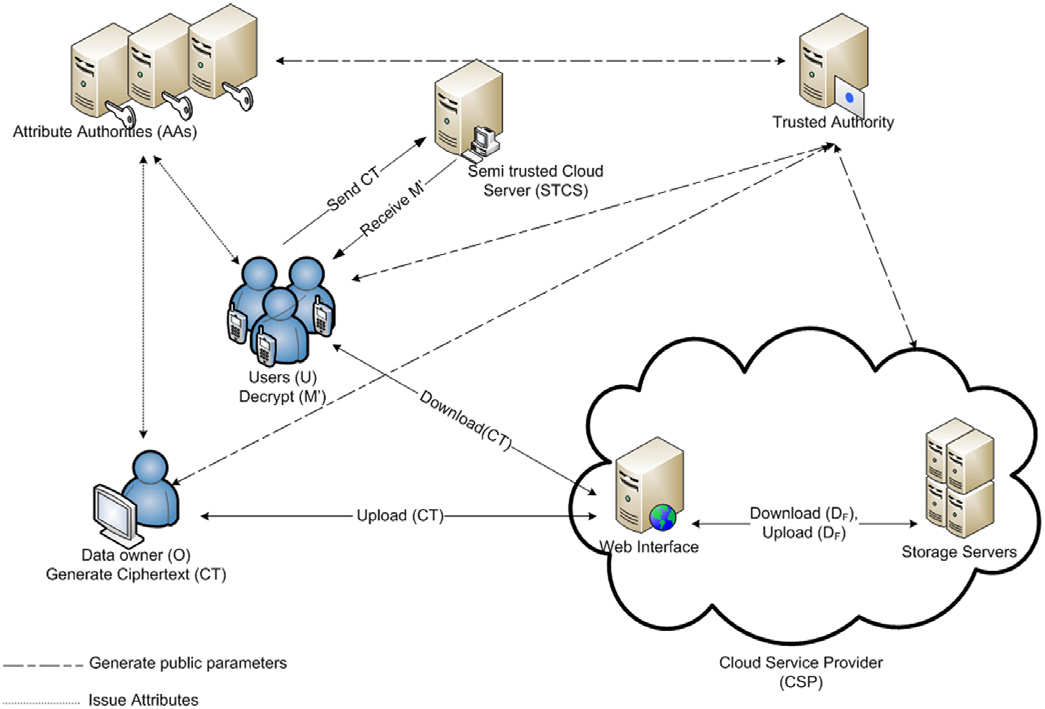
\includegraphics[width=0.8\textwidth]{phoabe-architecture}
		\caption{Architektur von PHOABE \cite{phoabe}}
	\end{figure}

	\subsection{Algorithmen}
	PHOABE besteht aus insgesamt sieben Algorithmen \cite{phoabe}. Es werden
	folgende Symbole für die Darstellung der Komponenten des Schemas verwendet.

	\begin{center}
	\begin{small}
		\begin{tabular}{p{3cm}p{9cm}}
			\hline
			Symbol & Beschreibung \\
			\hline
			STCS & Semi Trusted Cloud Server \\
			CTA & Central Trusted Authority \\
			$\lambda$ & Sicherheitsparameter \\
			$AA_j$ & Die $j$-te Attribute Authority \\
			$PP$ & Public Parameter \\
			$sk_{AA_j}$ & Der geheime Schlüssel der $j$-ten Attribute Authority \\
			$pk_{AA_j}$ & Der öffentliche Schlüssel der $j$-ten Attribute Authority \\
			$M_{pk}$ & Menge der öffentlichen Schlüssel aller Attribute Authorities \\
			$A$ & Zugriffsstruktur in LSSS-Matrix-Darstellung \\
			$\rho$ & Abbildung zum Auslesen einer Zeile von $A$ \\
			$p$ & Die Zugriffsregeln bestehend aus $p = \left(A, \rho\right)$ \\
			$C$ & Der aus der Nachricht erzeugte Geheimtext \\
			$GID$ & Die Identität eines Benutzers \\
			$S_{j, GID}$ & Menge von Attributen der $j$-ten Attibute Authority für den
			Benutzer mit der Identität $GID$ \\
			$sk_{j, GID}$ & Der geheime Schlüssel der $j$-ten Attribute Authority für
			den Benutzer mit der Identität $GID$ \\
			$M_{sk}$ & Menge von geheimen Schlüsseln $sk_{j, GID}$ der $j$-ten Attribute Authority \\
			$M_{tk}$ & Menge der Transformationsschlüssel $tk_{j, GID} \in M_{tk}$ \\
			$tpk_{j, GID}$ & Öffentlicher Transformationsschlüssel der $j$-ten
			Attribute Authority für den Benutzer mit der Identität $GID$ \\
			$tsk_{j, GID}$ & Geheimer Transformationsschlüssel der $j$-ten
			Attribute Authority für den Benutzer mit der Identität $GID$ \\
			$m$ & Die Nachricht \\
			$m'$ & Die teilweise entschlüsselte Nachricht vom STCS \\
			\hline
		\end{tabular}
	\end{small}
	\end{center}

	\newpage
	\begin{enumerate}
		\item \algitem{Setup}{}{\lambda}{PP} Der
			Setup-Algorithmus nimmt als Eingabe einen Sicherheitsparameter $\lambda$,
			liefert die öffentlichen Parameter $\text{PP}$ und wird von einer
			\textit{Central Trusted Authority} (CTA) ausgeführt.
		\item \algitem{Setup}{auth}{PP}{\left(sk_{AA_j}, pk_{AA_j}\right)} Bei $N$
			Autoritäten führt die Autorität $AA_j$ mit $j \in N$ diesen Algorithmus
			aus, um einen geheimen Schlüssel $sk_{AA_j}$ und einen öffentlichen
			Schlüssel $pk_{AA_j}$ zu generieren. Als Eingabe nimmt der Algorithmus die
			öffentlichen Umgebungsparameter $PP$.
		\item \algitem{Encrypt}{}{PP, M_{pk}, m, p}{C} Dieser Algorithmus
			ver\-schlüs\-selt die Nachricht $m$ unter Angabe einer Menge der
			öffent\-lich\-en Schlüssel $M_{pk} = \left\{ pk_{AA_j} \;\vert\; j \in N
			\right\}$. Jeder dieser Schlüssel werden von einer \textit{Attribute
			Authority} bereitgestellt. Zudem wird eine Zugriffsregel $p = \left( A,
			\rho \right)$ verwendet. Als Ausgabe wird ein Geheimtext $C$ erzeugt.
		\item\label{enum:phoabe_keygen} \algitem{Keygen}{}{PP, sk_{AA_j}, pk_{AA_j},
			GID, S_{j, GID}}{sk_{j, GID}} Dieser Algorithmus erzeugt einen privaten
			Schlüssel $sk_{j, GID}$ und wird von einer \textit{Attribute Authority}
			$AA_j$ ausgeführt. Der Schlüssel wird für einen Benutzer erzeugt und steht
			in Verbindung mit Attributen $S_{j, GID} = \left\{ a_1, ..., a_{n_j}
			\right\}$ der $AA_j$.  Dabei stellt $a \in S_{j, GID}$ ein Attribut und
			$n_j$ die Anzahl der Attribute von $AA_j$ dar. $GID$ ist die Identität vom
			Benutzer.
		\item \algitem{Transform}{}{PP, M_{sk}, p, C}{M_{tk}} Dieser Algorithmus
			wird von einem Benutzer ausgeführt. Dieser besitzt eine Menge von
			Attributen $S_{GID}$ und die dazugehörigen Schlüssel $M_{sk} = \left\{
			sk_{j, GID} \;\vert\; j \in N \right\}$. Die Schlüssel wurden vorher durch
			\textit{Attribute Authorities} für den Benutzer ausgestellt (siehe Punkt
			\ref{enum:phoabe_keygen}). Als Eingabe nimmt der Algorithmus zusätzlich
			die öffentlichen Parameter $PP$, die Zugriffsregel $p = \left(A,
			\rho\right)$ und den Geheimtext $C$. Als Ausgabe wird eine Menge von
			transformierten Schlüsseln $M_{tk} = \left( \left\{tpk_{j, GID} \;\vert\;
			j \in N\right\}, tsk_{GID} \right)$ erzeugt.
		\item \algitem{Decrypt}{out}{PP, M_{tk}, p, C}{m'} Dieser Algorithmus wird
			vom STCS ausgeführt und erzeugt die teilweise entschlüsselte Nachricht
			$m'$. Als Eingabe nimmt der Algorithmus die öffentlichen Parameter $PP$,
			eine Menge von transformierten Schlüsseln $M_tk$, die Zugriffsregeln $p =
			\left(A, \rho\right)$ und den Geheimtext $C$.
		\item \algitem{Decrypt}{}{m', tks_{GID}}{m} Dieser Algorithmus wird von
			Benutzer ausgeführt und nimmt als Eingabe die teilweise entschlüsselte
			Nachricht $m'$ und den geheimen Transformationsschlüssel $tsk_{GID}$. Als
			Ausgabe wird die Nachricht $m$ erzeugt.
	\end{enumerate}

	\newpage
	\bibliography{literatur}
	\bibliographystyle{abbrv}
\end{document}
